\chapter{Przyszłość Fundamentalnych Zasad}

Przeczytaliśmy już następujący cytat z rozdziału “\textit{Fundament Naszej Wiary}”. Jest to jedno z przewidywań Siostry White dotyczące wielkiej reformacji, która miała nastąpić wśród Adwentystów Dnia Siódmego; ta reformacja polegałaby na porzuceniu Fundamentalnych Zasad. Dokładnie w ten sposób zostanie ustanowiona nowa organizacja.

\egw{\textbf{Wróg dusz będzie starał się wprowadzić przypuszczenie, że wśród Adwentystów Dnia Siódmego miała nastąpić wielka reformacja, i że ta reformacja \underline{polegałaby na porzuceniu doktryn, które stoją jako filary naszej wiary} i zaangażowaniu się w proces reorganizacji}. Gdyby ta reformacja miała miejsce, co by z tego wynikło? \textbf{Zasady prawdy, które Bóg w swojej mądrości dał Kościołowi Ostatków, zostałyby odrzucone. Nasza religia zostałaby zmieniona. \underline{Fundamentalne zasady, które podtrzymywały dzieło przez ostatnie pięćdziesiąt lat, zostałyby uznane za błąd}}. \textbf{Zostałaby ustanowiona nowa organizacja. Zostałyby napisane książki nowego porządku. Zostałby wprowadzony system filozofii intelektualnej}. Założyciele tego systemu poszliby do miast i wykonaliby wspaniałą pracę. Szabat, oczywiście, byłby lekceważony, podobnie jak Bóg, który go stworzył. Nic nie mogłoby stanąć na drodze nowego ruchu. Przywódcy nauczaliby, że cnota jest lepsza od występku; ale \textbf{gdy Bóg zostałby usunięty}, \textbf{pokładaliby swoją ufność w ludzkiej mocy}, która bez Boga jest bezwartościowa. Ich fundament byłby zbudowany na piasku, a burza i nawałnica zmiotłyby tę konstrukcję.}[Lt242-1903.13; 1903][https://egwwritings.org/?ref=en\_Lt242-1903.13&para=7767.20]

\egwnogap{Kto ma autorytet, aby rozpocząć taki ruch? \textbf{Mamy nasze Biblie. Mamy nasze doświadczenie, potwierdzone cudownym działaniem Ducha Świętego}. \textbf{Mamy prawdę, która nie dopuszcza żadnego kompromisu.} \textbf{\underline{Czy nie powinniśmy odrzucić wszystkiego, co nie jest w harmonii z tą prawdą}?}}[Lt242-1903.14; 1903][https://egwwritings.org/?ref=en\_Lt242-1903.14&para=7767.21]

Ellen White widziała wysiłek wroga, aby usunąć te \emcap{Fundamentalne Zasady}. Podtrzymywały one dzieło od samego początku. Były to prawdy potwierdzone cudownym działaniem Ducha Świętego i nie dopuszczają one żadnego kompromisu. \egwinline{Czy nie powinniśmy odrzucić wszystkiego, co nie jest w harmonii z tą prawdą?}

\begin{figure}
    \centering
    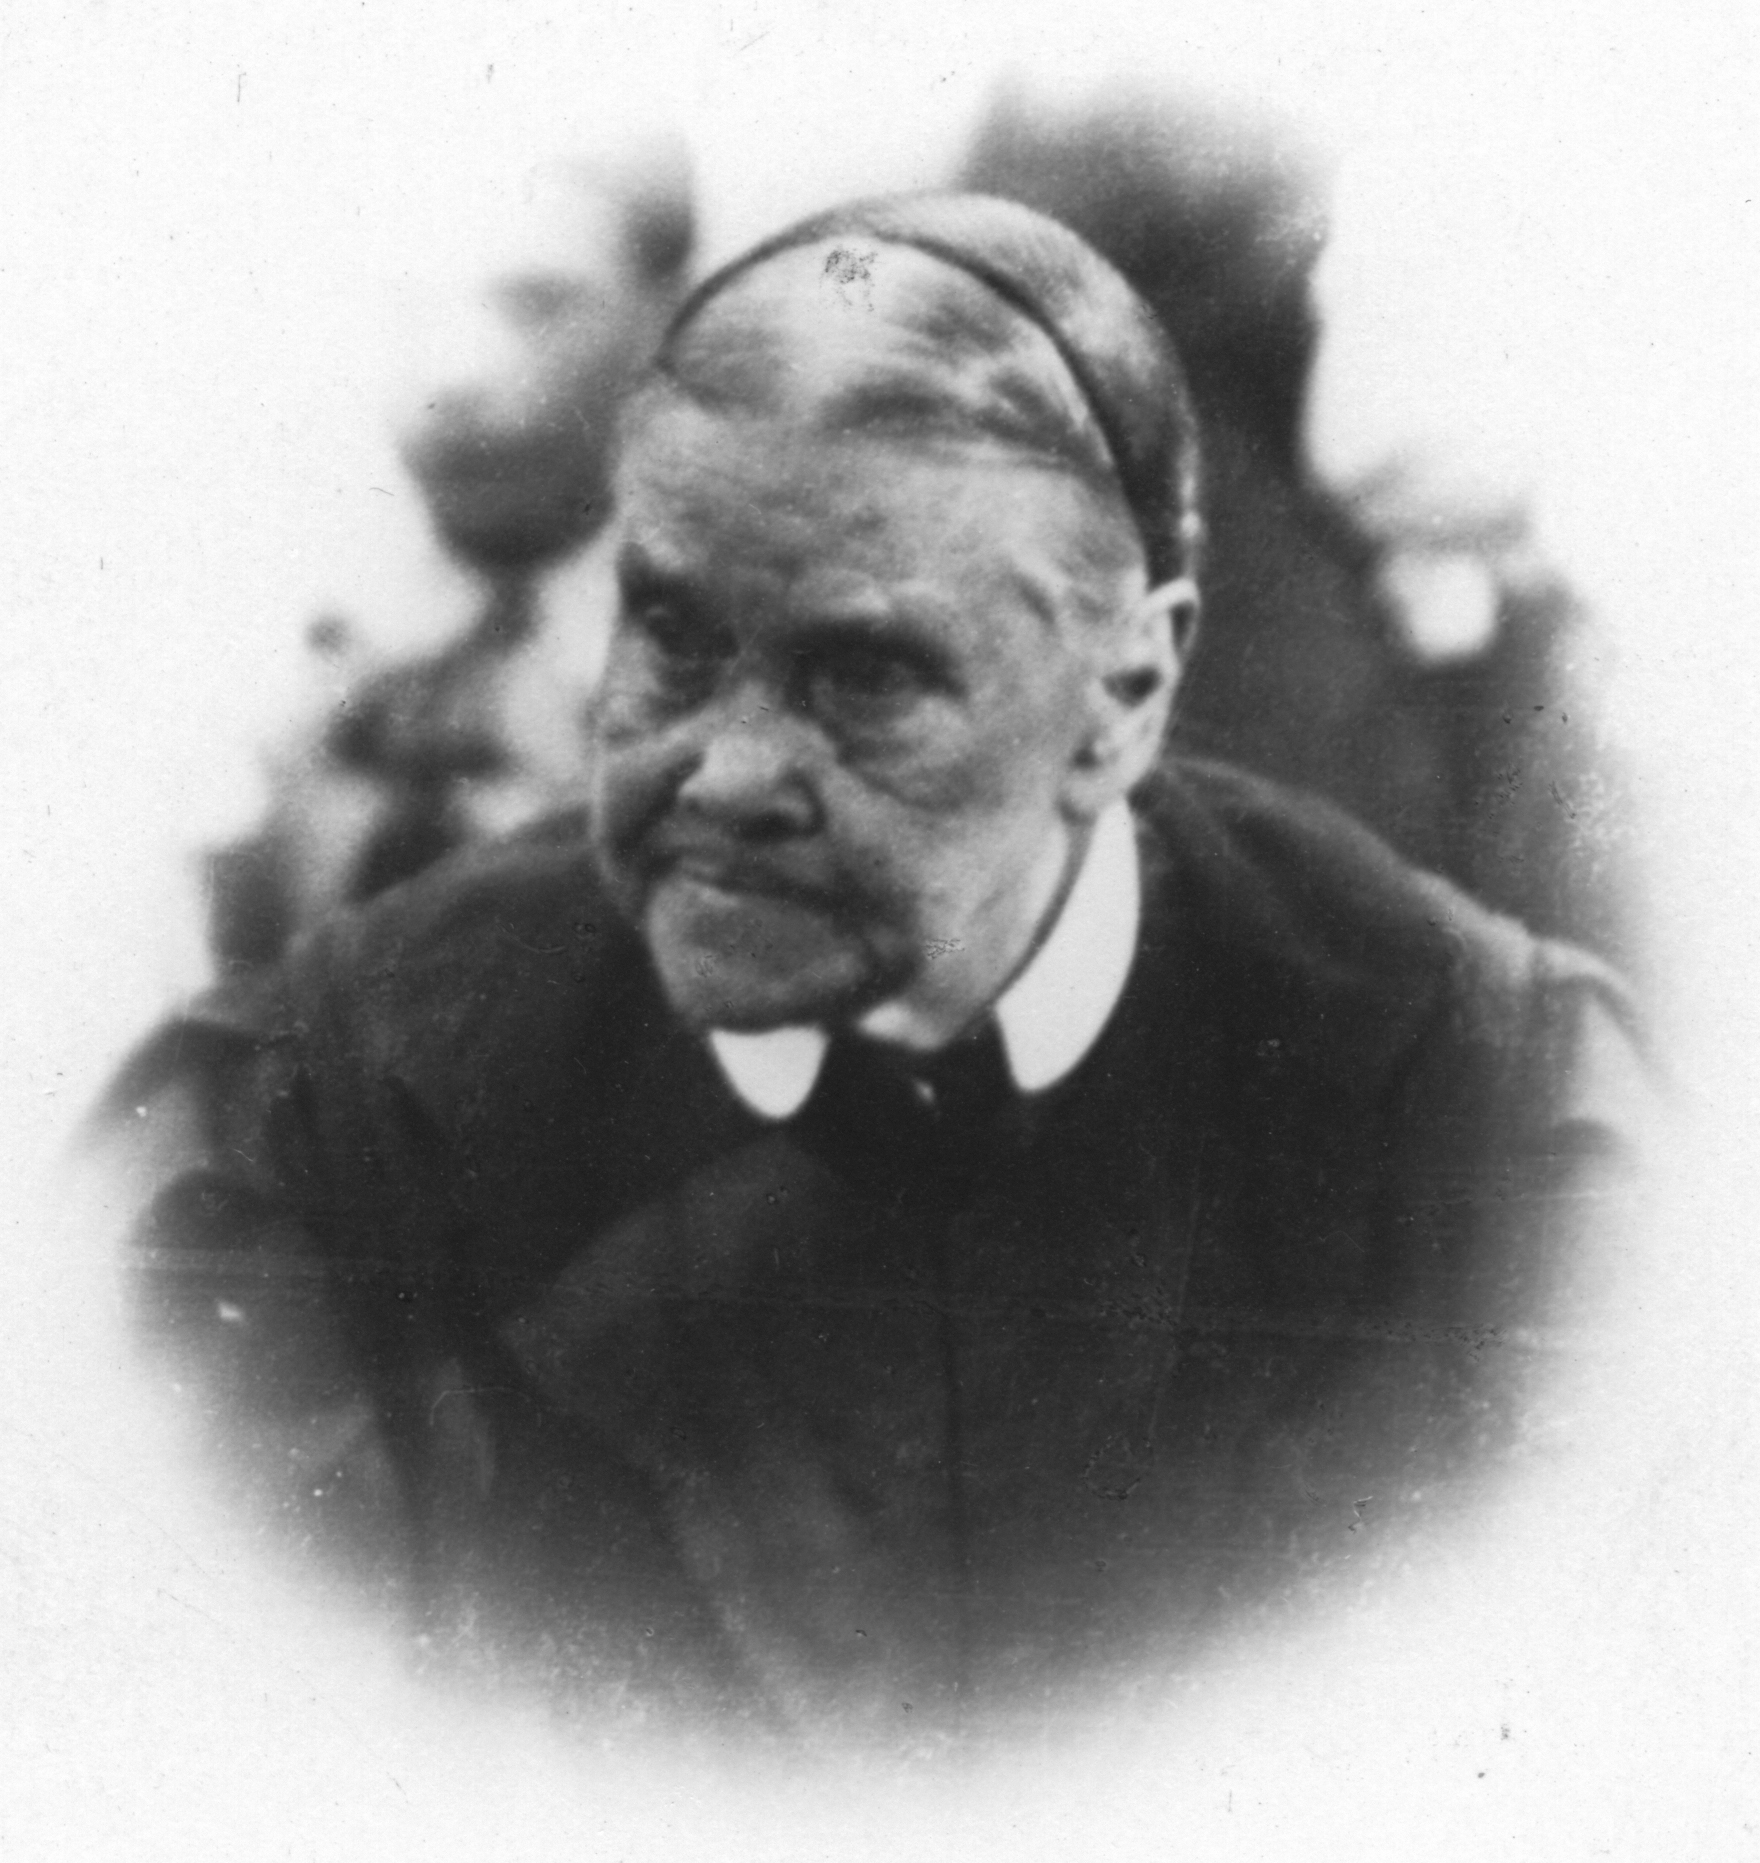
\includegraphics[width=1\linewidth]{images/ellen-white-1913.jpg}
    \caption*{Ellen G. White, 1913}
    \label{fig:e-white-1913}
\end{figure}

Siostra White przepowiedziała nam przyszłość. Dziś obserwujemy jej spełnienie. Porównując \emcap{Fundamentalne Zasady} z dzisiejszymi Fundamentalnymi Wierzeniami, widzimy, że nasza religia się zmieniła. Nasze przekonanie dotyczące \emcap{osobowości Boga} się zmieniło. Zostały napisane książki nowego porządku, które nie są oparte na solidnym Słowie Bożym. Został wprowadzony system filozofii intelektualnej.

Ta reformacja miała miejsce w jej czasach. Tak opisała dni Kościoła Adwentystów Dnia Siódmego w jej czasach i w przyszłości:

\egw{Obecny czas jest poważnym, pełnym trwogi czasem dla kościoła. Aniołowie są już przepasani, oczekując na rozkaz Boga, aby wylać swoje czasze gniewu na świat. Aniołowie zniszczenia podejmują dzieło zemsty, ponieważ Duch Boży stopniowo wycofuje się ze świata. Szatan również gromadzi swoje siły zła, wychodząc ‘do królów ziemi i całego świata’, aby zgromadzić ich pod swoim sztandarem, i przygotować do ‘bitwy w ów wielki dzień Boga Wszechmogącego.’ \textbf{Szatan podejmie najpotężniejsze wysiłki, aby zdobyć panowanie w ostatnim wielkim konflikcie. \underline{Fundamentalne zasady zostaną wydobyte na światło dzienne i zostaną podjęte decyzje w odniesieniu do nich}. Sceptycyzm przeważa wszędzie}. Bezbożność obfituje. \textbf{Wiara poszczególnych członków kościoła będzie poddana próbie, jakby nie było innej osoby na świecie}...}[Ms1a-1890.8; 1890][https://egwwritings.org/?ref=en\_Ms1a-1890.8&para=6780.13]

Najpotężniejsze wysiłki Szatana mają na celu usunięcie \emcap{Fundamentalnych Zasad} poprzez zasłonięcie ich sceptycyzmem. Oceniając z dzisiejszej perspektywy, poświadczamy prawdziwość proroctw Ellen White.

\egw{Mówię wam teraz, że kiedy zostanę złożona do grobu, \textbf{nastąpią wielkie zmiany}.}[Ms1-1915.2; 1915][https://egwwritings.org/?ref=en\_Ms1-1915.2&para=10771.9]

Prawdziwym pytaniem, które musimy sobie zadać  jest to: gdy \emcap{Fundamentalne Zasady} zostaną przedstawione, jaką decyzję podejmę w odniesieniu do nich? Czy nie powinniśmy odrzucić wszystkiego, co nie jest zgodne z tymi zasadami? Jaką decyzję podejmiesz?


% % The future of the Fundamental Principles

\begin{titledpoem}
    \stanza{
        In the early whisper of prophecy’s sound, \\
        Ellen White warned where dangers abound. \\
        "The enemy plots," she sternly declared, \\
        "To dismantle truths our forebears shared."
    }

    \stanza{
        Fundamental Principles, strong and sure, \\
        Once the bedrock, pure and unpure. \\
        Now the sands shift beneath our creed, \\
        Where new doctrines grow like wayward weed.
    }

    \stanza{
        Reformation masked as light so bright, \\
        Undermines the pillars, eroding right. \\
        Books rewritten, philosophies anew, \\
        Skepticism veils what once we knew.
    }

    \stanza{
        Shall the Sabbath lose its sacred glow? \\
        Shall we forget the God that we owe? \\
        "The foundation crumbles," so it seems, \\
        As truth is lost to intellectual dreams.
    }

    \stanza{
        Look back to the days, to the Spirit-led start, \\
        Where divine truths were etched in heart. \\
        Satan’s strategies, cunning and keen— \\
        Eroding what once was clearly seen.
    }

    \stanza{
        So, brethren, now to the past return, \\
        To the roots of faith, let our hearts yearn. \\
        For the warnings spoken, the visions seen, \\
        Call us to defend what they truly mean.
    }

    \stanza{
        Stand firm in the storm as the tempests roar, \\
        Reclaim the truths worth fighting for. \\
        Ellen’s voice echoes, stark and clear: \\
        "Repudiate the false, hold the righteous near."
    }

    \stanza{
        Make your choice, as the battle lines draw, \\
        On the side of the timeless, divine law. \\
        To the Fundamental Principles, fiercely hold, \\
        The original faith, courageous and bold.
    }
\end{titledpoem}

% \begin{titledpoem}

    \stanza{
        Proroctwa wczesny jeszcze głos \\
        Przewidział, jaki będzie los. \\
        „Diabeł ma spisek nam przeciwny, \\
        By wykraść prawdy w sposób dziwny”.
    }

    \stanza{
        Zasady, które niegdyś były, \\
        Które od Boga pochodziły, \\
        Na piasku teraz się ruszają, \\
        Bo ludzie Boga nie słuchają.
    }

    \stanza{
        Idee przebrane za światło, \\
        Usunąć filary tak łatwo. \\
        Książki też były przepisane, \\
        Nowe teorie nauczane.
    }

    \stanza{
        Czy szabat też mamy porzucić \\
        I tak od Boga się odwrócić? \\
        „Podstawy runą” — tak się zdaje, \\
        Gdy duma w miejsce prawdy staje.
    }

    \stanza{
        Wspomnijcie, jak żeśmy zaczęli, \\
        Gdy żeśmy prawdę w sercach mieli. \\
        Lecz poprzez podstępy szatana \\
        Teraz już prawda jest niechciana.
    }

    \stanza{
        Powróćmy zatem do przeszłości, \\
        Do wczesnej wiary i wierności, \\
        Bo miał zapewnić głos proroczy, \\
        Że z dobrej ścieżki nikt nie zboczy.
    }

    \stanza{
        Przetrwajmy burzę, która trwa, \\
        Gdyż warta tego prawda ta. \\
        Głosowi Ellen więc uwierzmy \\
        I prawdę drogą tak wybierzmy.
    }

    \stanza{
        A zanim przyjdzie na świat trwoga, \\
        Ustawmy się po stronie Boga. \\
        Ze starych ścieżek nie zbaczajmy \\
        I zepchnąć z nich się już nie dajmy.
    }

\end{titledpoem}
